\chapter{Cinética Química}

\section{Introdução à Cinética}

A cinética é o ramo que estuda velocidade reação e os fatores que a influenciam. Dentre alguns
fatores que serão abordados incluem: pressão, temperatura, concentração, catalisadores, etc. O
estudo da cinética não é algo fácil, pois envolve diversos fatores que tem de ser levados em conta,
muitas vezes sendo necessárias estudos laboratoriais, faixa desejada, para que seja entendido a
reação. \par

\section{Reação Química: Definições e Classificações}

Uma reação química pode ser definida como um rearranjo ou redistribuição de átomos de uma ou mais
moléculas, resultando em outra com propriedades físicas e químicas diferentes. \par

Quanto a suas classificações podemos dividi-las em:
\begin{itemize}
    \item { Quanto á fase em que ocorre:
        \begin{enumerate}
            \item Reações homogêneas: são aquelas em que os reagentes e/ou produtos estão na mesma fase.
            \item {Reação heterogêneas: aquelas em que as espécies químicas estão em fases diferentes}
        \end{enumerate}
    }
    \item {Quanto à estequiometria
        \begin{enumerate}
            \item {Reações Simples: são aquelas que apresenta uma única estequiometria para as substâncias
            reagentes diante de qualquer modificação nas condições de processo}
            \item {Reações múltiplas: são aquelas que apresentam mais de uma estequiometria para as substâncias
            reagentes diante de qualquer modificação nas condições de processo}\
        \end{enumerate}
    }
    \item {Quanto ao número de etapas:
        \begin{enumerate}
            \item {Reações elementares: são aquelas que ocorrem em uma única etapa}
            \item {Reações complexas: são aquelas que ocorrem em mais de uma etapa}
        \end{enumerate}
    }
\end{itemize}
%Fim da seção de classificação de reações químicas
%────────────────────────────────────────────────────────────────────────────────────────────────────────────────────────────────────────────────────
\section{Fatores que influenciam a velocidade de reação}
Alguns fatores que influenciam a velocidade de reação são:
\begin{itemize}
    \item {Concentração dos reagentes: Quanto mais moléculas reagentes por unidade de volume, maior
    será a taxa de colisão entre elas, gerando uma mor velocidade de reação.}
    \item {Pressão: Aumentando a pressão, aumenta-se o contato entre os reagentes, pois eles serão
    forçados a ficarem mais juntos, aumentando a taxa de colisões efetivas entre os reagentes, aumentando
    a velocidade reação.}
    \item {Natureza dos reagentes: Para que se tenha uma reação química, é necessário a quebra de
    ligações existentes entre os átomos dos reagentes, e a formação de novas ligações entre os átomos
    que serão formados. Portanto, se precisar quebrar mais ligações e as ligações são fortes,
    necessariamente nossa reação será mais lenta.}
    \item {Superfície de contato: A superfície de contato é a área efetiva entre um reagente e
    outro. Como necessariamente as reações químicas dependem de colisões, uma maior área de contato 
    implica em uma maior velocidade de reação.}
    \item {Luz e eletricidade: Algumas reações químicas são influenciadas pela luz e eletricidade,
    de forma que se forem expostas a um desses fatores, uma reação fotoquímica, para luz, ou uma
    reação eletroquímica, para eletricidade, maior a velocidade de reação.}
    \item {Temperatura: Sendo a temperatura uma medida do grau de agitação das moléculas, se
    introduzirmos um aumento de temperatura e consequentemente um aumento da energia cinética, mais 
    facilmente, ou com maior probabilidade, as moléculas se chocarão e causarão uma reação química.}
    \item {Catalisadores: A presença de um catalisador é para aumentar a velocidade de reação, seja 
    facilitando a quebra de ligações químicas, seja formando complexos que aumentam a facilidade da reação.
    Um catalisador não pode ser consumido durante a reação e não pode sofrer alteração na sua
    composição.}
\end{itemize}
%Fim da seção de fatores que influenciam a velocidade de reação
%────────────────────────────────────────────────────────────────────────────────────────────────────────────────────────────────────────────────────
\section{Velocidade de reação}
A velocidade de reação química pode ser definida tanto pela taxa de consumo de reagentes, quanto
pela taxa de produção de produtos. Como se trata de uma taxa, a velocidade de reação é definida pela
letra \(r\) com o subscrito do reagente ou produto a qual está se referindo. Similarmente, o sinal
negativo indica consumo, ou seja, ele é um reagente e o positivo indica produção, ou seja, ele é um
produto. \par 

As relações entre as velocidades de uma reação são dadas quando se aplica a estequiometria da reação
quando vamos relacionar as velocidades. Ou seja, para uma dada reação
\[
\ch{aA + bB -> cC + dD}
\]
Onde a relação entre as velocidades pode ser dada por
\begin{equation}
    \frac{\left( -r_{A} \right) }{a} = \frac{\left( -r_{B} \right) }{b} = \frac{\left( r_{C} \right) }{c} = \frac{\left( r_{D} \right) }{d} = \mathbf{r}
\end{equation}
Onde \(\mathbf{r}\) é a velocidade de reação. \par

Se tivermos a unidade de velocidade reação em \(\frac{mol}{L.s}\), podemos dizer que que são
consumidos ou produzidos \(\frac{mol}{L}\) por segundo. Portanto, em um reator com um volume \(V\)
tem uma taxa de reação dada por:
\begin{equation}\label{tax_reacao_reator}
    \frac{\mathrm{d}N_A}{\mathrm{d}t} = r_AV
\end{equation}
Mas com as ressalvas que para que isso seja verdade o conteúdo do reator precisa ser homogêneo, com
mesma temperatura, concentrações e velocidades de reação. Outra ressalva é o cuidado quanto aos
sinais negativos, onde dentro de um balanço, pode ver que apareça um sinal negativo a frente de um
reagente. Isso significa que ele está sendo consumido, com sua produção sendo negativa. \par
%Fim da seção de velocidade de reação
%────────────────────────────────────────────────────────────────────────────────────────────────────────────────────────────────────────────────────
\section{Tempo de meia-vida e tempo infinito.}
O tempo de meia vida é aquele necessário para que metade do reagente limitante seja consumido. Já o
tempo infinito é aquele necessário para que se atinja o equilíbrio químico da reação, ou seja, não
terá mais variações significativas nas concentrações dos reagentes e produtos. \par
%Fim da seção de tempo de meia-vida e tempo infinito
%────────────────────────────────────────────────────────────────────────────────────────────────────────────────────────────────────────────────────
\section{Lei da Ação das Massas de Guldberg-Waage}
A lei da ação das massas de Guldberg-Waage é uma lei empírica que relaciona a velocidade de reação
com a concentração dos reagentes. Ela é dada por:
\begin{equation}
    \left( -r_A \right) = k C_A^{\alpha}C_B^{\beta}
\end{equation}
Onde \(k\) é a constante de velocidade, \(\alpha\) e \(\beta\) são os expoentes de ordem parcial
da reação, e \(C_A\) e \(C_B\) são as concentrações dos reagentes. Temos que a ordem global da reação,
\(n\) é a soma desses expoentes de ordem parcial, ou seja, \(\alpha + \beta = n\). \par
%Fim da seção de lei da ação das massas de Guldberg-Waage, explicação para as reações

\subsection{Reações Elementares}
Para reações elementares, experimentalmente foi verificado que as ordens parciais coincidem com os
coeficientes estequiométricos, por exemplo, para decomposição do Rádio, temos
\[
\ch{1Ra -> 1Rn + 1He}
\]
Possui velocidade de reação, para o rádio igual a 
\begin{equation}
    \left( -r_{Ra} \right) = k C_{Ra}^1
\end{equation}
Onde o expoente de ordem parcial é igual ao coeficiente estequiométrico. \par
%Fim da seção de reações elementares
\subsection{Reações não-elementares}
Considerando uma reação de oxidação do ferro, temos
\[
\ch{5Fe^2+ + MnO4^- + 8H^+ -> 5Fe^3+ + Mn^2+ + 4H2O} 
\]
A reação é altamente improvável de ocorrer em uma única etapa, mas ela pode ser descrita através de
uma série de reações elementares \footnote{Isso será explicado em capítulos posteriores.}. \par

Para um exemplo mais concreto, temos o rearranjo de decomposição do \ch{CH3CHO} em \ch{CH4CO}, que
apresenta uma velocidade de reação dada por:
\[
\left( - r_{\ch{CH3CHO}} \right) = k C_{\ch{CH3CHO}}^{\frac{2}{3}}
\] 
Sendo que ela não corresponderia a algo elementar, já que não segue o padrão observado
anteriormente. \par
%Fim da seção de reações não-elementares
\subsection{Molecularidade}
Esse conceito é amplamente utilizado para classificação de reações elementares. Ele é definido como o
número de moléculas que reagem em uma etapa elementar. \par
\begin{table}[H]
\centering
\begin{tabular}{c|c|c}
\toprule
Reação & Molecularidade &  Classificação \\
 \midrule
 \ch{A -> B} & 1 &  Unimolecular \\
 \ch{A + B -> C} & 2 &  Bimolecular \\
 \ch{A + B + C -> D} & 3 &  Trimolecular \\
\bottomrule
\end{tabular}
\caption{Molecularidade de Reações}
\label{tab:molecularidade}
\end{table}
%Fim da seção de molecularidade
%────────────────────────────────────────────────────────────────────────────────────────────────────────────────────────────────────────────────────
\section{Lei de Arrhenius}
De acordo com a lei de Boltzmann a fração de colisões entre moléculas reagentes, cuja excedem a
energia \(E\), que é a energia de ativação, é igual a \(\exp^{  \left( (- \frac{E}{RT}) \right)} \). De
acordo com Arrhenius, somente as moléculas ativadas promoveriam a reação, portanto, a velocidade de
reação deveria ser proporcional à fração de moléculas que são ativadas, logo
\begin{equation}
    k = A \exp ^{\left( -\frac{E}{RT} \right)}  
\end{equation}
Onde \(A\) é a frequência de colisão, e \(E\) é a energia de ativação. \par

As unidades das constantes de velocidade variam de acordo com a ordem da reação, por exemplo, para
uma reação de primeira ordem, a unidade de \(k\) é \(\frac{1}{s}\), já para uma reação de segunda
ordem, a unidade de \(k\) é \(\frac{1}{mol \cdot s}\). \par
%Fim da seção de lei de Arrhenius
%────────────────────────────────────────────────────────────────────────────────────────────────────────────────────────────────────────────────────
\section{Exercícios}\
\subsection{Exercício 1}
Uma reação dada por \ch{1A + 3B -> C + 2D} teve suas velocidades iniciais registradas abaixo
\begin{table}[H]
\centering
\begin{tabular}{c|c|c}
\toprule
\(C_{A0} \; \frac{mol}{l}\)  & \(C_{B0} \;  \frac{mol}{l}\)  & \(\left( -r_{A0}  \right) \; \frac{mol}{Ls} \)    \\
 \midrule
 \(0.1\)  & \(0.1\)   &   \(0.5\) \\
 \(0.1\)  &  \(0.2\)  &  \(1.0\)  \\
 \(0.2\)  & \(0.1\)  & \(2\)   \\
\bottomrule
\end{tabular}
\caption{Velocidades de reação}
\label{tab:ex1_tabela_vel}
\end{table}
Determine a equação de velocidade e o valor da velocidade específica desta reação.
\subsection{Resolução}
Quando a concentração do reagente \(B\) é dobrada, a velocidade também é dobrada, porém, quaando se
dobra a concentração do reagente \(A\), a velocidade é quadruplicada, logo, a ordem da reação em 
relação ao reagente \(A\) é igual a \(2\), e a ordem da reação em relação ao reagente \(B\) é igual
a \(1\). Nossa equação fica então
\begin{equation}
    \left( -r_A \right) = k C_A^2 C_B
\end{equation}
Para acharmos o valor de \(k\), basta substituirmos os valores de concentração e velocidade na
equação acima:
\begin{align}
    \left( -r_A \right) &= k C_A^2 C_B \\
    0.5 &= k \cdot 0.1^2 \cdot 0.1 \\
    k &= 500 \; \frac{L^{2} }{mol^{2}  \cdot s}
\end{align}
%Fim da resolução do exercício 1
%────────────────────────────────────────────────────────────────────────────────────────────────────────────────────────────────────────────────────

\subsection{Exercício 2}
Um estudo realizado sobre uma determinada substância foi realizado e chegou-se na seguinte tabela
\begin{table}[H]
\centering
\begin{tabular}{c|c|c|c|c|c|c}
\toprule
T \(\degree C\)  & \(2\)  & \(10\)  &\(20\)   & \(25\)  & \(35\)  &  \(40\)  \\
 \midrule
\(k \; \frac{1}{s}\)   & \(0.0126\) & \(0.017\)   &\(0.020\)   &\(0.027\)   &\(0.028\)   &\(0.038\)    \\
\bottomrule
\end{tabular}
\caption{Constantes de Velocidade para diferentes temperaturas}
\label{tab:ex2_tabela_temp}
\end{table}
Determine a energia de ativação e o fator de frequência para essa reação.
\subsection{Resolução}
Para determinarmos a energia de ativação e o fator de frequência, devemos utilizar a equação de
Arrhenius. Como temos uma tabela, podemos lineariza-la para facilitar o cálculo. Para isso, vamos
aplicar o logaritmo natural em ambos os lados da equação de Arrhenius:
\begin{align}
    k &= A \exp ^{\left( -\frac{E}{RT} \right)} \\
    \ln k &= \ln A \exp ^{\left( -\frac{E}{RT} \right)} \\
    \ln k &= \ln A - \frac{E}{RT} \\
    \ln k &= \ln A - \frac{E}{R} \cdot \frac{1}{T}
\end{align}
Agora, podemos linearizar a equação acima, fazendo \(y = \ln k\), \(a = \ln A\) e \(b =
-\frac{E}{R}\) e \(x = \frac{1}{T}\). Realizando a linearização em python, com o seguinte código:
\begin{minted}[linenos]{python}
import numpy as np
import matplotlib.pyplot as plt
from scipy import stats

T = np.array([2, 10, 20, 25, 35, 40]) + 273.15
k = np.array([0.0126, 0.017, 0.020, 0.027, 0.028, 0.038])

y = np.log(k)
x = 1/T

slope, intercept, r_value, p_value, std_err = stats.linregress(x,y)

print("slope: %f    intercept: %f" % (slope, intercept))
print("R-squared: %f" % r_value**2)
fig = plt.figure()
ax = fig.add_subplot()
ax.plot(x, y, 'o', label='Dados Originais')
ax.plot(x, intercept + slope*x, 'r', label='Linha de regressão')
plt.xlabel(r'$\frac{{1}}{{T}}$')
plt.ylabel(r'$\ln(k)$')
ax.text(0.52, 0.77, r'$\ln(k) = -\frac{E_a}{R} \frac{1}{T} + \ln(A)$', fontsize=15,
         transform=ax.transAxes)
ax.text(0.52, 0.70, r'$y = {} + {}x$'.format(round(intercept, 4),
                                             round(slope, 4)), fontsize=15,
                                            transform=ax.transAxes)
ax.text(0.52, 0.63, r'$R^2 = {}$'.format(round(r_value**2, 4)), fontsize=15,
                                            transform=ax.transAxes)
plt.legend()
plt.show()
\end{minted}
Obtemos o seguinte gráfico:
\begin{figure}[H]
    \centering
    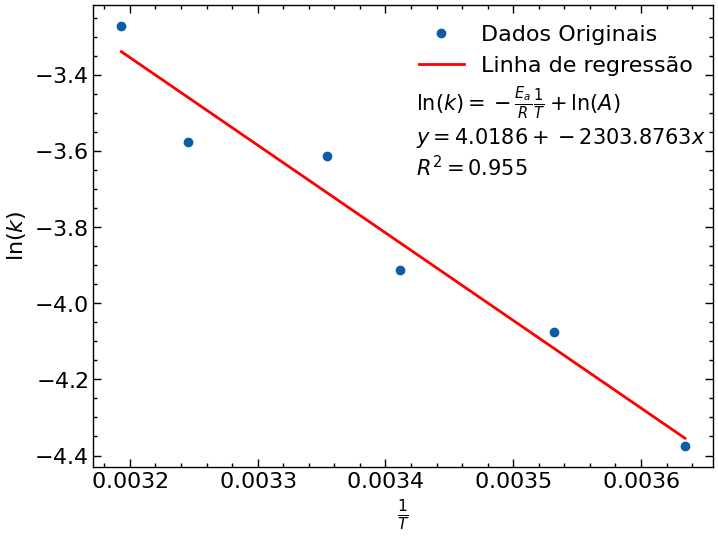
\includegraphics[width=0.8\textwidth]{ex2_grafico}
    \caption{Gráfico da linearização da equação de Arrhenius}
    \label{fig:ex2_grafico}
\end{figure}
E os seguintes valores para os parâmetros:
\begin{align}
    a &= \ln A = 4.014 \\
    b &= -\frac{E}{R} = 2301
\end{align}
Portanto, nosso valor da energia de ativação é \(E = 2301 \cdot 8.314 = 19130 \; \frac{J}{mol}\) e
nosso valor de \(A\) é \(A = \exp ^{4.014} = 55.368 \; \frac{1}{s}\). 
%────────────────────────────────────────────────────────────────────────────────────────────────────────────────────────────────────────────────────
%Começo do Capítulo 2 na apostila dele
\section{Reações de Pseudo-Primeira Ordem}
Seja uma reação qualquer, dada por
\begin{equation}
    \ch{A + B -> C }
\end{equation}
Onde a taxa de reação é dada por:
\begin{equation}
    \left( -r_A \right) = k C_A C_B
\end{equation} 
Reações de segunda ordem geram expressões bastantes complexas, bem mais que aquelas de primeira
ordem. Uma forma fácil de simplificação para resolução de exercícios é tratá-la como uma reação de
pseudo-primeira ordem, trabalhando com um grande excesso de um dos reagentes. \par

Supondo na reação enunciada acima que tivéssemos 0.5 mols de \(A\) e 100 mols de \(B\), ao final da
reação, a concentração de \(B\) quase não teria variação, podendo ser tratada como constante. Logo,
se tivermos um reator com volume \(V\), \(B\) teria uma concentração \(C_B = \frac{N_{B0} }{V}\).
Podemos definir uma constante pseudo-cinética, \(k^{\prime} \), dada por:
\begin{equation}
    k^{\prime} = k C_B 
\end{equation}
Podemos definir nossa velocidade para a reação de pseudo-primeira ordem como:
\begin{equation}
    \left( -r_A \right) = k^{\prime} C_A
\end{equation}
Essa aproximação só é válida se um dos reagentes exceder em pelo menos 20 vezes a concentração do
outro reagente.  \par
%────────────────────────────────────────────────────────────────────────────────────────────────────────────────────────────────────────────────────
\section{Equilíbrio Químico}
A diversas reações químicas que são reversíveis e para qual a velocidade de formação dos reagentes a
partir da formação dos produtos vai aumentando com o tempo, devido ao aumento da concentração dos
produtos. Seja a reação elementar dada por:
\begin{equation}
    \ch{A <=> B}
\end{equation}
Sabendo que a reação direta apresenta uma constate de velocidade \(k_d\) e a inversa uma constante
de velocidade \(k_i\). A par que a reação ocorre, a concentração de \(A\) diminui e a de \(B\)
aumenta. Isso faz com que se tenha uma variação de velocidade ao longo da reação, a par que as
concentrações vão mudando a velocidade muda proporcionalmente. \par

No equilíbrio, as velocidades de reação sao iguais, ou seja, a velocidade da reação direta é igual a
velocidade da reação inversa, portante, podemos afirmar que as concentrações se mantém constantes.
No estudo dessas reações, é importante saber como é a variação de um determinado reagente no meio
reacional. Na reação anteriormente mencionada, temos que o valor \(\left( -r_{A}  \right) \) é dado
por:
\begin{equation}
    \left( -r_{a} \right) = \left( -r_A \right)_d - \left( +r_A \right)_i 
\end{equation}

Onde temos que o reagente é consumido durante a reação direta e produzido durante a reação inversa.
Por estequiometria, temos que a taxa de produção de \(A\) na reação inversa é a mesma de consumo de
\(B\), logo podemos reescrever a equação acima como:
\begin{equation}
    \left( -r_{a} \right) = \left( -r_A \right)_d - \left( -r_B \right)_i 
\end{equation}
Onde, substituindo as equações de velocidade, temos:
\begin{equation}
    \left( -r_{a} \right) = k_d C_A - k_i C_B
\end{equation}
Para o equilíbrio, temos que \(\left( -r_{a} \right) = 0\), logo:
\begin{equation}
    \frac{k_d}{k_i} = \frac{C_{Be} }{C_{Ae} } = K_c
\end{equation}
Onde \(K_c\) é a constante de equilíbrio. Os índices \(e\) indicam que são as concentrações no
equilíbrio. \par
Assim, a constante de equilíbrio é determinada pelas concentrações de equilíbrio dos reagentes e
produtos. Para uma reação \(\ch{A + 2B <=> 3C + D}\), nossa constante de equilíbrio é dada por:
\begin{equation*}
    K_c = \frac{C_{Ce}^3 C_{De} }{C_{Ae} C_{Be}^2}
\end{equation*} 
Porém, essa relação só é válida para reações elementares, para reações não-elementares. Para a
reação não elementar abaixo, temos que:
\begin{equation}
    \ch{3ClO- <=> ClO3- + 2Cl-}
\end{equation}
A constante de equilíbrio é dada por:
\begin{equation}
    K_c = \frac{C_{ClO_3^-} C_{Cl^-}^2}{C_{ClO^-}^3}
\end{equation}
Porém, essa reação é composta de duas reações elementares, que são:
\begin{align*}
    \ch{2ClO- &<=>[k_1][k_{1,Inv}] ClO2- + Cl-}
    \ch{ClO2- + ClO- &<=>[k_2][k_{2,Inv}] ClO3- + Cl-}
\end{align*}
No equilíbrio, as velocidades das reações diretas e inversas são iguais, logo:
\begin{align*}
    k_1 C_{\ch{ClO}_{e}}^{2} = k_{1,Inv} C_{\ch{ClO2}_{e}} C_{\ch{Cl-}_{e}} \\
    k_2 C_{\ch{ClO2-}_{e}}C_{\ch{ClO-}_{e}} = k_{2,Inv} C_{\ch{ClO3-}_{e}} C_{\ch{Cl-}_{e}}
\end{align*}
Dividindo a primeira equação pela segunda, temos:
\begin{equation}
    \frac{k_1}{k_2} \frac{C_{\ch{ClO}_{e}}^{2}}{C_{\ch{ClO2-}_{e}}C_{\ch{ClO-}_{e}}} = \frac{k_{1,Inv}}{k_{2,Inv}} \frac{C_{\ch{ClO2-}_{e}} C_{\ch{Cl-}_{e}}}{C_{\ch{ClO3-}_{e}} C_{\ch{Cl-}_{e}}}
\end{equation}
Onde, isolamos as constantes de velocidade e as concentrações de equilíbrio, temos:
\begin{equation}
    \frac{k_1 k_2}{k_{1,Inv} k_{2,Inv}} = \frac{C_{\ch{ClO3-}_{e}}C_{\ch{Cl-}_{e}}}{C_{\ch{ClO2-}_{e}}}
\end{equation}
%────────────────────────────────────────────────────────────────────────────────────────────────────────────────────────────────────────────────────
\section{Reações em Fase Gasosa}
Para uma reação em fase gasosa elementar qualquer, temos:
\begin{equation}
    \ch{A + B -> C}
\end{equation}
Onde a velocidade de reação é dada por:
\begin{equation}
    \left( -r_A \right)^{\star} =k^{\star} P_A P_B
\end{equation}
Em termos das pressões parciais dos nossos gases. Poderíamos escrever em função da concentração,
também seria totalmente valido, porem, para gases, é mais comum trabalhar com pressão. \par

Nota-se também que os valores que seriam obtidos por \(\left( r_A \right) \) e \(\left( r_A
\right)^{\star} \) serão diferentes, similarmente como as constantes de velocidade \(k\) e
\(k^{\star} \) também são. \par

A constante \(k^{\star} \) é a constante de velocidade em termos de pressão parcial, existindo uma
correlação com \(k\) que dependerá da ordem de reação,. Se aplicarmos a equação de Clapeyron ao
reagente \(A\), temos:

\begin{align}
    P_A V &= n_A R T \\
    C_A &= \frac{n_A}{V} =  \frac{P_A}{RT} \\
\end{align}
O processo é o mesmo para o reagente \(B\). Substituindo na nossa equação de velocidade, temos:
\begin{align}
    \left( -r_A \right)^{\star} &= k^{\star} P_A P_B \\
    \left( -r_A \right)^{\star} &= k^{\star} C_A C_B \left( RT \right)^2 \\
    \frac{\left( -r_A \right)^{\star}}{RT} &= k^{\star} C_A C_B RT
    \frac{\left( -r_A \right)^{\star}  }{RT} &= \left( -r_A \right) 
\end{align}
Onde a relação entre as constantes de velocidade é \(k = k^{\star} RT\) válida para reações de
segunda ordem. Em fato, a depender da ordem, a formula geral para conversão é dada por
\begin{equation}
    k = k^{\star} \left( RT \right)^{n-1}
\end{equation}
Onde \(n\) é a ordem da reação. \par
%Fim da seção de reações em fase gasosa
%────────────────────────────────────────────────────────────────────────────────────────────────────────────────────────────────────────────────────
\section{Exercícios}
\subsection{Exercício 1}
A reação \ch{A + B -> C + D} foi estudada em laboratório e as concentrações dos reagentes foram
monitoradas ao longo do tempo, dando a seguinte tabela:
\begin{table}[H]
\centering
\begin{tabular}{c|c|c|c|c|c|c}
\toprule
Tempo (min) & 0 & 10 & 30 & 60 & 90 &  120 \\
 \midrule
 \(C_A\) \(\frac{mol}{L}\)  & 1 & 0.8 & 0.6 & 0.5 & 0.4 &  0.35 \\
 \(C_B\) \(\frac{mol}{L}\)  & 20 & 19.8 & 19.6 & 19.5 & 19.4 &  19.35 \\
\bottomrule
\end{tabular}
\caption{Tempo e concentração dos Reagentes}
\label{tab:cap2_ex1_tabela}
\end{table}
Sabendo que ela é elementar e possui \(k = 2.5 \; \frac{mol}{L \cdot  min}\), verifique se ela pode
ser tratada como de pseudo-primeira ordem. Faça o grafico de \(\left( -r_A \right) \) por \(t\)
\subsection{Resolução}
Vamos determinar as reações de velocidade para o reagente \(A\), considerando como reação de segunda
ordem e pseudo-primeira ordem, respectivamente:
\begin{align}
    \left( -r_A \right) &= 2.5 \cdot C_A \cdot C_B \\
    \left( -r_A \right) &= 2.5 \cdot C_A \cdot 20 = 50 \cdot C_A
\end{align}
O gráfico é feito pelo python pelo seguinte código:
\begin{minted}[linenos]{python}
import numpy as np
import matplotlib.pyplot as plt

t = np.array([0, 10, 30, 60, 90, 120])
Ca = np.array([1, 0.8, 0.6, 0.5, 0.4, 0.35])
Cb = np.array([20, 19.8, 19.6, 19.5, 19.4, 19.35])

ra_seg = 2.5 * Ca * Cb
ra_pse = 50 * Ca

fig = plt.figure()
ax = fig.add_subplot()
ax.plot(t, ra_seg, 'o', label='Segunda Ordem')
ax.plot(t, ra_pse, 'o', label='Pseudo-Primeira Ordem')
plt.xlabel(r'$t \; (min)$')
plt.ylabel(r'$\left( -r_A \right) \; \frac{{mol}}{{L \cdot min}}$')
plt.legend()
plt.show()
\end{minted}
Resultando no seguinte gráfico
\begin{figure}[H]
    \centering
    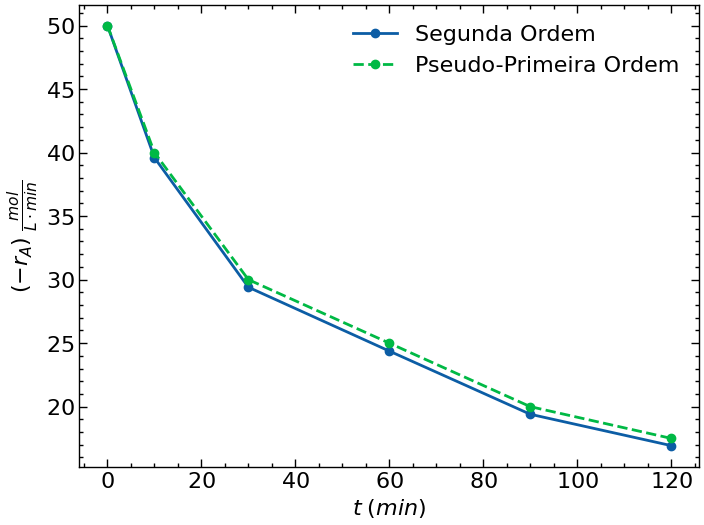
\includegraphics[width=0.8\textwidth]{cap2_ex1_grafico}
    \caption{Gráfico de \(\left( -r_A \right) \) por \(t\)}
    \label{fig:cap2_ex1_grafico}
\end{figure}
%Fim da resolução do exercício 1
%────────────────────────────────────────────────────────────────────────────────────────────────────────────────────────────────────────────────────
\subsection{Exercício 2}
Seja a reação não elementar \ch{H2O2 + H+ + I- <=> H2O + HOI}. Sabendo que ela pode ser representada
pelos seguintes passos elementares:
\begin{align*}
    \ch{H+ + I- &<=>[k_1][k_{1,Inv}] HI} \\
    \ch{HI + H2O2 &<=>[k_2][k_{2,Inv}] H2O + HOI} \\
\end{align*}
Onde \(k_1 = 0.0023, \; K_{1, Inv} = 0.44, \; k_2 = 1.03 \cdot 10^{-4}, \; k_{2, Inv} = 22 \), todas
em \(\frac{L}{mol \cdot min}\). Determine o valor de \(k_{c} \) 
\subsection{Resolução}
No equilíbrio, nossas reações inversas e diretas tem a mesma taxa de reação, logo:
\begin{align*}
    k_1 C_{\ch{H+}_{e}} C_{\ch{I-}_{e}} &= k_{1,Inv} C_{\ch{HI}_{e}} \\
    k_2 C_{\ch{HI}_{e}} C_{\ch{H2O2}_{e}} &= k_{2,Inv} C_{\ch{H2O}_{e}} C_{\ch{HOI}_{e}} \\
\end{align*}
Multiplicando as equações, vamos ter:
\begin{align*}
    k_1 k_2 C_{\ch{H+}_{e}} C_{\ch{I-}_{e}} C_{\ch{HI}_{e}} C_{\ch{H2O2}_{e}} &= k_{1,Inv} k_{2,Inv} C_{\ch{HI}_{e}} C_{\ch{H2O}_{e}} C_{\ch{HOI}_{e}} \\
    \frac{k_1 k_2}{k_{1,Inv} k_{2,Inv}} &= \frac{C_{\ch{H2O}_{e}} C_{\ch{HOI}_{e}}}{C_{\ch{H+}_{e}} C_{\ch{I-}_{e}} C_{\ch{HI}_{e}} C_{\ch{H2O2}_{e}}} \\
    K_c &= \frac{C_{\ch{H2O}_{e}} C_{\ch{HOI}_{e}}}{C_{\ch{H+}_{e}} C_{\ch{I-}_{e}} C_{\ch{H2O2}_{e}}} \\
\end{align*}
Ou seja, nossa constante de equilíbrio tem valor de
\begin{equation*}
    k_{c} = \frac{1.03 \cdot 10^{-4} \cdot 0.0023}{0.44 \cdot 22} = 2.44731 \cdot 10^{-8}
\end{equation*}
%Fim da resolução do exercício 2
%────────────────────────────────────────────────────────────────────────────────────────────────────────────────────────────────────────────────────
\subsection{Exercício 3}
A reação hipotética \ch{A => 2B} com um \(k = 278 \; \frac{L^{2} }{mol ^{2} s}\). Escreva a equação
de velocidade para essa reação em termos de concentração e em termos de pressão parcial. 
\subsection{Resolução}
Primeiramente será necessário realizar análise dimensional da nossa concentração.
\begin{align*}
    \left( -r_A \right) &= k C_A^n \\
    \left( \frac{mol}{L \cdot s} \right) &= \left( \frac{L^{2}}{mol ^{2} s}  \right)  \left( \frac{mol^{3}}{L^{3} } \right)      
\end{align*}
Portanto, nossa concentração tem unidade de \(\frac{mol^{3} }{L^{3} }\), com \(n = 3\). NOssa reação
é de terceira ordem. Portanto, para achar \(k^{\star} \) aplicamos a formula
\begin{align*}
    k &= k^{\star} \left( RT \right)^{n-1} \\
    278 &= k^{\star} \left( 8.314 \cdot 298 \right)^{3-1} \\
    k^{\star} &= 0.454 \; \frac{1}{atm^{2} \cdot s}
\end{align*} 
Portanto, nossa equação fica
\begin{equation*}
    \left( -r_A \right)^{\star} = 0.454 \cdot P_A^3
\end{equation*}
%Fim da resolução do exercício 3
%────────────────────────────────────────────────────────────────────────────────────────────────────────────────────────────────────────────────────
%Inicio do capitulo 3 na apostila dele
%to do
\section{Estequiometria Cinética-Conversão}
A conversão, geralmente denotada pela letra \((X_n)\) indica a quantidade que foi reagida em relação
a quantidade inicial que tínhamos. Será utilizado a letra \(A\) para o reagente limitante. Portanto,
para o limitante, temos \(X_A\) de conversão, variando de \(0 \to 1\). Considere a reação
genérica \ch{aA + bB -> cC + dD}, ocorrendo em batelada em um determinado reator. Indicamos o índice
\(0\)  como sendo para o instante inicial. Ou seja, no instante inicial teríamos \(n_{A0} \) mols de
\(A\), \(n_{B0} \) mols de \(B\), \(n_{C0} = 0\) mols de \(C\) e \(n_{D0} = 0\) mols de \(D\). \par

\begin{figure}[ht]
	\centering
	\caption{}
	%\incsvg{path/}{path/file}
	\incsvg{Materias/Imagens}{Materias/Imagens/Reator_Batelada}\\
	\label{fig:Reator_Batelada}
\end{figure}

Quando não colocamos índice, estamos indiciando que é num instante \(t\) qualquer de tempo. A
conversão do nosso reagente limitante é dada por:
\begin{equation}
    X_A = \frac{n_{A0} - n_A}{n_{A0} }
\end{equation}
%────────────────────────────────────────────────────────────────────────────────────────────────────────────────────────────────────────────────────
\subsection{Tabela Estequiométrica}
Considerando os coeficientes da reação genérica anterior, temos a seguinte tabela:
\begin{table}[H]
\centering
\begin{tabular}{c|c|c|c|c|c}
\toprule
 & \ch{aA} & \ch{bB} & \ch{->} & \ch{cC} &  \ch{dD} \\
 \midrule
 Início & \(N_{A0}\)  & \(N_{B0}\)  &  & \(N_{C0}\)  &  \(N_{D0}\)  \\
 Variação & \(-N_{A0} X_A\)  & \(-\frac{b}{a}N_{A0}X_A\)  &  & \(\frac{c}{a}N_{A0}X_A\)  & \(\frac{d}{a} N_{A0}X_A\)   \\
 Restante &  \(N_{A0} - N_{A0} X_A\)  & \(N_{B0} - -\frac{b}{a}N_{A0}X_A\)  &  & \(N_{C0} - \frac{c}{a}N_{A0}X_A\)  &  \(N_{D0} - \frac{d}{a} N_{A0}X_A \)  \\
\bottomrule
\end{tabular}
\caption{Tabela Estequiométrica Genérica}
\label{tab:tablea_estequiometrica}
\end{table}

Para um instante \(t\) qualquer, temos a seguinte fórmula para a quantidade presente no reator:
\begin{equation}
    N_{i} = N_{A0} \left( \frac{N_{i0} }{N_{A0} } + \gamma_i \frac{i}{a}X_A \right)  
\end{equation}
Onde \(i\) é o índice do reagente ou produto e \(\gamma_i\) é um operador que possui valores dados
abaixo
\begin{equation}
    \begin{dcases}
    1, &\text{ se } \text{Produto} ;\\
    -1, &\text{ se } \text{Reagente} ;\\
    \end{dcases}
\end{equation}

Importante que essas formulas são validas para qualquer tempo, porém, nãos oferecem relação nenhuma
para saber o tempo da reação.\par
%────────────────────────────────────────────────────────────────────────────────────────────────────────────────────────────────────────────────────
\section{Variações de Concentração}
Como o número de mols varia com tempo, não é nada distante imaginar que a concentração também
variará em função do tempo. Basta pegar pela própria definição de concentração \(C_A =
\frac{N_A}{V}\). Vale ressaltar que essa formula apenas é válida quando todas as espécies estão
igualmente distribuídas no volume do reator. \par

\subsection{Reações a Volume Constantes}  
Se conduzirmos nossa reação em um reator fechado e de paredes rígidas, podemos admitir que o volume
se manterá constante. Similarmente, se fizermos uma reação apenas com fases líquidas, não é muito
distante pensar que o volume se manterá constante. Sendo assim, podemos considerar \(V = V_0\), ou
seja, nossas equações de concentração ficam:

\begin{equation}\label{eq:cap3_concentracao_volume_fixo}
    C_i = C_{A0} \left( \frac{N_{i0}}{N_{A0} } + \gamma_i \frac{i}{a}X_A \right)  
\end{equation}

Geralmente, para produtos, temos que \(N_{C0} = N_{D0} = 0 \), podendo simplificar um pouco nossas
equações. 

\subsection{Reações a Volume Variável}
Quando temos reações a volume variável, ou seja, em fases gasosas, reator contínuo ou em batelada de
parede móvel, temos que a concentração varia com o tempo. Podemos considerar, em fases gasosa, o
volume reacional com função do número  total de mols através da equação de Clapeyron:

\begin{equation}
    V = \frac{n R T}{P} = \frac{\left( N_A + N_B + N_C + N_D \right) RT}{P}
\end{equation}

Podemos simplificar essa equação, substituindo os valores de \(N_i\) em função de \(X_A\), temos:

\begin{equation}
    V = \left[N_{A0} \left( 1 + \frac{N_{B0} }{N_{A0}} + \frac{N_{C0} }{N_{A0}} + \frac{N_{D0} }{N_{A0}}\right) + N_{A0}\frac{d+c-b-a}{a}X_A \right] \frac{RT}{P}
\end{equation}

Definindo a grandeza 

\begin{equation}
    y_{A0} = \frac{N_{A0} }{N_{T0}}
\end{equation}

Onde \(N_{T0} = N_{A0} + N_{B0} + N_{C0} + N_{D0} \) é o número total de mols no instante inicial.
Substituído de volta na equação anterior, temos:

\begin{equation}
    V = \left( N_{T0} + y_{A0} N_{T0} \frac{d+c-b-a}{a}X_A \right) \frac{RT}{P}
\end{equation}

A fração de conversão volumétrica é dada por:

\begin{equation}
    \varepsilon _A = y_{A0} \delta  
\end{equation}

Onde \(\delta = \frac{d+c-b-a}{a}\). A fração de conversão volumétrica é também conhecida como o
fator  de expansão, indicando o quanto o sistema se expande ou contrai durante a reação. \par

Substituindo de volta na equação anterior, temos:

\begin{equation}
    V = \left( 1 + y_{A0} \delta X_A \right) N_{T0} \frac{RT}{P}    
\end{equation}

Podemos utilizar a equação de Clapeyron para a condição inicial

\begin{equation}
    N_{T0} = \frac{P_0 V_0}{RT_0}
\end{equation}

Com isso, temos:

\begin{equation}
    V = \left( 1 + \varepsilon_A X_A \right) \frac{P_{0} T }{P T_0}
\end{equation}

Com isso, para nossas concentrações, temos:

\begin{equation}\label{eq:cap3_concentracao_volume_variavel}
    C_i = \frac{C_{A0}\left( \frac{N_{i0}}{N_{A0} } +\gamma_i \frac{i}{a}X_A\right)}{\left( 1 + \varepsilon_A X_A \right) \frac{P_0T}{PT_0} }
\end{equation}
%────────────────────────────────────────────────────────────────────────────────────────────────────────────────────────────────────────────────────
\section{Exercícios}
\subsection{Exercício 1}
A reação \ch{H2 + Cl2 -> 2HCl} é realizada em fase gasosa a 5 atm em um reator de paredes móveis com
concentrações iniciais de \(C_{H2} = 3 \; \frac{mol}{L} \) e \(C_{Cl2} = 4 \; \frac{mol}{L} \).
Determine
\begin{enumerate}
    \item O reagente limitante \label{item:cap3_ex1_item1}
    \item A concentração de \ch{Cl2} no tempo de meia vida da reação \label{item:cap3_ex1_item2}
    \item A pressão parcial de \ch{HCl} apos \(70 \%\) de conversão \label{item:cap3_ex1_item3}
    \item {Se \(73 \; \frac{g}{L}\) de \ch{HCl} estiverem presentes no início da reação, qual sera
    sua conversão se sua concentração atingir \(146 \; \frac{g}{L}\) \label{item:cap3_ex1_item4}}
\end{enumerate}
\subsection{Resolução}
\subsubsection{Item \ref{item:cap3_ex1_item1}}
Para determinar qual irá ser o limitante, vamos analisar a quantidade alimentada \textit{vs} a
quantidade estequiométrica necessária para a reação. Temos que:
\begin{equation*}
    \ch{1H2 + 1 Cl2 -> 2HCL}
\end{equation*}
Temos que nossas quantias estequiométricas são 1 mol de \ch{H2} para 1 mol de \ch{Cl2}. Portanto,
aquele com menor quantia será o limitante, no nosso caso, será o \ch{H2}.

\subsubsection{Item \ref{item:cap3_ex1_item2}}

Conforme estabelecido \(A\) é tratado como o reagente limitante. Como foi dito que, a reação é
gasosa e em paredes móveis, temos que usar a equação \refeq{eq:cap3_concentracao_volume_variavel}.
Portanto, para o \ch{Cl2}, temos:

\begin{equation*}
    C_{Cl2} = \frac{C_{A0} \left( \frac{N_{Cl20}}{N_{A0} } - \frac{1}{1}X_A \right)}{\left( 1 + \varepsilon_A X_A \right) \frac{P_0T}{PT_0} }
\end{equation*}

Porém, temos que

\begin{align*}
    \delta &= \frac{c - b - a}{a}\\
    &= \frac{2 - 1 - 1}{1}
    &= 0
\end{align*}

Considerando nossa reação como isotérmica e à pressão constante, nossa equação se reduz a

\begin{equation*}
    C_{Cl2} = C_{A0} \left( \frac{N_{Cl20}}{N_{A0} } - \frac{1}{1}X_A \right)
\end{equation*}

Onde o tempo de meia vida é dado por \(X_A = 0.5\). Substituindo os valores, temos:

\begin{align*}
    C_{Cl2} &= 3 \left( \frac{4}{3} - \frac{1}{1} \cdot 0.5 \right) \\
    &= 2.5 \; \frac{mol}{L}
\end{align*}

\subsubsection{Item \ref{item:cap3_ex1_item3}}

Fazendo as mesmas correlações para o produto, nossa formula se reduz a:

\begin{equation*}
    C_{HCl} = C_{A0} \left( \frac{N_{HCl0}}{N_{A0}} + \frac{2}{1}X_A \right)
\end{equation*}

Multiplicando nossa equação por \(RT\), temos:

\begin{align*}
    C_{HCl} = C_{A0} RT \left( \frac{N_{HCl0}}{N_{A0}} + 2 X_A \right)
    P_C = P_{A0} \left( \frac{N_{HCl0}}{N_{A0}} + 2 X_A \right)
\end{align*}

Sabendo que \(P_{A0}  = y_{A0} P\), temos

\begin{align*}
    P_C = P_{A0} \left( \frac{N_{HCl0}}{N_{A0}} + 2 X_A \right)
\end{align*}
